% TikZ figures included from SHIFA_SYSTEM_TECHNICAL_DESCRIPTION.tex
% Requires: \usepackage{tikz}, positioning, arrows.meta, shapes.geometric, calc, backgrounds, fit

\newcommand{\ShifaFigSystemContext}{%
\begin{figure}[!htbp]
\centering
\begin{tikzpicture}[
  font=\small\sffamily,
  node distance=6mm and 10mm,
  client/.style={rounded corners=2pt, draw=blue!60!black, thick, fill=blue!6, minimum width=2.8cm, minimum height=1.1cm, align=center},
  core/.style={rounded corners=3pt, draw=teal!70!black, very thick, fill=teal!10, minimum width=3.4cm, minimum height=1.3cm, align=center},
  data/.style={rounded corners=2pt, draw=orange!70!black, thick, fill=orange!8, minimum width=2.6cm, minimum height=0.95cm, align=center},
  ext/.style={rounded corners=2pt, draw=gray!60, dashed, fill=gray!12, minimum width=2.2cm, minimum height=0.75cm, align=center, font=\scriptsize\sffamily},
  arr/.style={-{Stealth[length=2.2mm]}, thick}
]
\node[client] (p) {Patient app\\\scriptsize\texttt{shifa\_patient\_app\_v1}};
\node[client, right=2.4cm of p] (d) {Doctor / Admin app\\\scriptsize\texttt{shifa\_doc\_app\_v1}};
\path (p.south) -- coordinate[midway] (midtop) (d.south);
\node[core, below=1.1cm of midtop] (api) {Backend API\\\scriptsize\texttt{shifa-doctor-backend}};
\node[data, below=0.9cm of api] (db) {PostgreSQL};
\node[ext, left=1.5cm of api] (fb) {Firebase\\Auth / FCM};
\node[ext, right=1.5cm of api] (daily) {Daily.co\\video};
\node[ext, below=0.5cm of daily] (ai) {OpenAI\\(AI features)};
\draw[arr] (p.south) -- ++(0,-0.35) -| (api.north west);
\draw[arr] (d.south) -- ++(0,-0.35) -| (api.north east);
\draw[arr] (api) -- (db);
\draw[arr, dashed] (fb.east) -- (api.west);
\draw[arr, dashed] (daily.west) -- (api.east);
\draw[arr, dashed] (ai.west) -- ++(-0.6,0) |- (api.east);
\end{tikzpicture}
\caption{High-level system context: two Flutter clients, one Spring Boot API, PostgreSQL, and main external integrations.}
\label{fig:system-context}
\end{figure}%
}

\newcommand{\ShifaFigPatientNav}{%
\begin{figure}[!htbp]
\centering
\begin{tikzpicture}[
  font=\small\sffamily,
  tab/.style={rounded corners, draw, minimum width=1.85cm, minimum height=0.65cm, align=center},
  shell/.style={rounded corners, draw=teal!60, thick, inner sep=6pt},
  lbl/.style={font=\scriptsize\itshape}
]
\node[shell, label=above:\textbf{StatefulShellRoute (indexedStack)}] (ss) {
\begin{tikzpicture}[node distance=3mm]
\node[tab, fill=teal!10] (h) {Home};
\node[tab, fill=teal!10, right=of h] (b) {Bookings};
\node[tab, fill=teal!10, right=of b] (doc) {Docs};
\node[tab, fill=teal!10, right=of doc] (dr) {Doctors};
\end{tikzpicture}};
\node[shell, below=8mm of ss, label=above:\textbf{ShellRoute + bottom bar}] (sh) {
\begin{tikzpicture}[node distance=3mm]
\node[tab, fill=gray!15] (a) {Account};
\node[tab, fill=gray!15, right=of a] (c) {Chat};
\node[tab, fill=gray!15, right=of c] (n) {Notif.};
\node[tab, fill=gray!15, right=of n] (t) {Tasks};
\end{tikzpicture}};
\node[tab, fill=red!12, dashed, thick, below=8mm of sh, minimum width=6cm] (v) {Video call (fullscreen, no bottom bar)};
\node[lbl, left=2mm of ss.west, align=right] {GoRouter};
\end{tikzpicture}
\caption{Patient app navigation: four primary tabs preserve state per branch; account/chat/notifications/tasks share another shell; video is outside shells.}
\label{fig:patient-nav}
\end{figure}%
}

\newcommand{\ShifaFigDoctorShell}{%
\begin{figure}[!htbp]
\centering
\begin{tikzpicture}[
  font=\small\sffamily,
  sb/.style={rounded corners, draw, fill=teal!50!black, text=white, minimum width=1.15cm, minimum height=0.55cm, inner sep=2pt, font=\scriptsize},
  main/.style={draw, rounded corners, minimum width=5.2cm, minimum height=3.2cm, align=left, inner sep=8pt}
]
\node[sb, anchor=north west] (n0) at (0,0) {Chat};
\node[sb, below=3pt of n0.south west, anchor=north west] (n1) {Home};
\node[sb, below=3pt of n1.south west, anchor=north west] (n2) {Cal.};
\node[sb, below=3pt of n2.south west, anchor=north west] (n3) {Patients};
\node[sb, below=3pt of n3.south west, anchor=north west] (n4) {Tasks};
\node[sb, below=3pt of n4.south west, anchor=north west] (n5) {Bell};
\node[sb, below=3pt of n5.south west, anchor=north west] (n6) {Profile};
\node[main, anchor=north west, xshift=1.35cm, yshift=0.1cm] (content) at (0,0) {\textbf{Nested Navigator}\\[0.25em]
\scriptsize Appointments, patients, task details, etc.};
\draw[thick] (1.22,0.15) -- (1.22,-3.45);
\end{tikzpicture}
\caption{Doctor \texttt{MainShell}: vertical sidebar (schematic) and inner \texttt{Navigator} for stacked routes.}
\label{fig:doctor-shell}
\end{figure}%
}

\newcommand{\ShifaFigBackendLayers}{%
\begin{figure}[!htbp]
\centering
\begin{tikzpicture}[
  font=\small\sffamily,
  layer/.style={rounded corners, draw, minimum width=6.8cm, minimum height=1.0cm, align=center},
  arr/.style={-{Stealth}, thick}
]
\node[layer, fill=blue!8] (w) {\textbf{web} --- REST controllers (\texttt{/api/...})};
\node[layer, fill=green!10, below=5mm of w] (s) {\textbf{service} --- business rules, transactions};
\node[layer, fill=yellow!15, below=5mm of s] (r) {\textbf{repo} --- Spring Data JPA};
\node[layer, fill=orange!12, below=5mm of r] (d) {\textbf{domain} --- entities + \texttt{@Entity}};
\node[layer, fill=gray!20, below=5mm of d] (db) {PostgreSQL};
\draw[arr] (w) -- (s);
\draw[arr] (s) -- (r);
\draw[arr] (r) -- (d);
\draw[arr] (d) -- (db);
\end{tikzpicture}
\caption{Backend layering in \texttt{com.shifa}: controllers delegate to services, repositories, and JPA entities.}
\label{fig:backend-layers}
\end{figure}%
}

\newcommand{\ShifaFigJwtFlow}{%
\begin{figure}[!htbp]
\centering
\resizebox{\textwidth}{!}{%
\begin{tikzpicture}[
  font=\small\sffamily,
  scale=0.94,
  actor/.style={rounded corners, draw, minimum height=0.75cm, minimum width=2.2cm, align=center},
  jwtbox/.style={rectangle, draw, rounded corners, inner sep=4pt, align=center, font=\scriptsize},
  arr/.style={-{Stealth[length=2mm]}, thick}
]
\node[actor] (c) {Client};
\node[jwtbox, right=1.2cm of c] (a) {POST \texttt{/api/auth/login}};
\node[jwtbox, right=1.0cm of a] (j) {JWT + session record};
\node[jwtbox, right=1.0cm of j] (r) {Bearer on API calls};
\draw[arr] (c) -- (a);
\draw[arr] (a) -- (j);
\draw[arr] (j) -- (r);
\node[jwtbox, below=1.0cm of j, text width=5.6cm, align=left, fill=red!5] (note) {Admin scope: optional \texttt{?app=} query on login\\(doctor client stores admin\\JWT separately).};
\end{tikzpicture}%
}
\caption{Simplified authentication flow\\
(see \texttt{AuthController},\\
\texttt{JwtAuthFilter}).}
\label{fig:jwt-flow}
\end{figure}%
}

\newcommand{\ShifaFigSecurityRisk}{%
\begin{figure}[!htbp]
\centering
\begin{tikzpicture}[
  font=\small\sffamily,
  bad/.style={rounded corners, draw=red!70!black, very thick, fill=red!8, align=left, text width=6.2cm, inner sep=6pt},
  arr/.style={-{Stealth}, thick, red!60!black}
]
\node[bad] (box) {
\textbf{Risk: unauthenticated file access}\\
\scriptsize\texttt{SecurityConfig}: \texttt{/patientdocuments/**} $\rightarrow$ \texttt{permitAll}\\
\scriptsize\texttt{PatientDocumentFileController} + \texttt{StaticResourceConfig}\\serve files by path.};
\node[bad, below=6mm of box, fill=orange!10] (mit) {\scriptsize Mitigation direction: signed URLs, auth on download, opaque object keys,\\never rely on secrecy of filenames.};
\draw[arr] (box) -- (mit);
\end{tikzpicture}
\caption{Document URL exposure (code-derived): treat as high severity until redesigned.}
\label{fig:security-risk}
\end{figure}%
}

\newcommand{\ShifaFigDeployment}{%
\begin{figure}[!htbp]
\centering
\begin{tikzpicture}[
  font=\small\sffamily,
  box/.style={rounded corners, draw, minimum width=2.8cm, minimum height=0.85cm, align=center, font=\scriptsize},
  arr/.style={-{Stealth}, thick}
]
\node[box, fill=blue!8] (gh) {Git repo\\(no CI in tree)};
\node[box, fill=teal!15, right=1.5cm of gh] (rw) {Railway build\\\texttt{gradlew -x test}};
\node[box, fill=teal!20, right=1.2cm of rw] (jar) {JVM + JAR};
\node[box, fill=orange!12, below=1.0cm of jar] (fb) {Firebase Hosting\\doctor + admin SPA};
\node[box, fill=purple!10, left=1.5cm of fb] (flt) {\texttt{flutter build web}};
\draw[arr] (gh) -- (rw);
\draw[arr] (rw) -- (jar);
\draw[arr, dashed] (flt) -- (fb);
\end{tikzpicture}
\caption{Deployment signals from repository files: backend ships via Railway-style Gradle build; doctor web via Flutter then Firebase Hosting.}
\label{fig:deployment}
\end{figure}%
}

\newcommand{\ShifaFigTestBars}{%
\begin{figure}[!htbp]
\centering
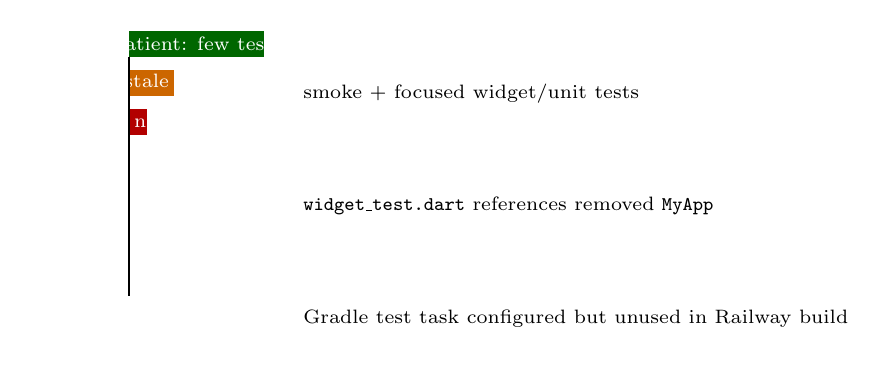
\begin{tikzpicture}[
  font=\small\sffamily,
  scale=0.95
]
\begin{scope}[x=0.12cm,y=0.35cm]
\fill[green!40!black] (0,0) rectangle (15,1) node[midway, text=white, font=\scriptsize] {Patient: few tests};
\fill[orange!80!black] (0,-1.5) rectangle (5, -0.5) node[midway, text=white, font=\scriptsize] {Doctor: stale template};
\fill[red!70!black] (0,-3) rectangle (2, -2) node[midway, text=white, font=\scriptsize] {Backend: no src/test};
\end{scope}
\draw[thick] (0,0) -- (0,-3.2);
\node[anchor=west, font=\scriptsize] at (2.2,-0.5) {smoke + focused widget/unit tests};
\node[anchor=west, font=\scriptsize] at (2.2,-2) {\texttt{widget\_test.dart} references removed \texttt{MyApp}};
\node[anchor=west, font=\scriptsize] at (2.2,-3.5) {Gradle test task configured but unused in Railway build};
\end{tikzpicture}
\caption{Qualitative automated test coverage as inferred from repository structure (not line coverage).}
\label{fig:test-bars}
\end{figure}%
}
